../cictikz/src/cictikz/data/tex/cictikz_preamble.tex

% Reverse biased pn junction as a varactor: the depletion region is the
% dielectric, its width moves with the reverse voltage, and the
% capacitance follows the inverse square root.

\begin{tikzpicture}[thick]

  \definecolor{preg}{RGB}{240,120,110}
  \definecolor{nreg}{RGB}{60,80,220}

  % junction bar
  \fill[preg!45] (0,0) rectangle (3.4,2.2);
  \fill[nreg!55] (5.35,0) rectangle (9.0,2.2);
  \draw (0,0) rectangle (9.0,2.2);
  \node[anchor=center] at (1.5,1.1) {p$-$};
  \node[anchor=center, white] at (7.5,1.1) {n$+$};

  % depletion region: ionized acceptors left, donors right of the junction
  \draw[densely dotted, black!60] (4.7,0) -- (4.7,2.2);
  \foreach \y in {0.4,1.1,1.8} {
    \foreach \x in {3.7,4.25} {
      \draw[nreg] (\x,\y) circle (0.14);
      \draw[nreg] ({\x-0.08},\y) -- ({\x+0.08},\y);
    }
    \foreach \x in {5.0} {
      \draw[red] (\x,\y) circle (0.14);
      \draw[red] ({\x-0.08},\y) -- ({\x+0.08},\y);
      \draw[red] (\x,{\y-0.08}) -- (\x,{\y+0.08});
    }
  }

  % depletion width
  \draw[<->] (3.4,-0.35) -- (5.35,-0.35);
  \node[anchor=north] at (4.4,-0.45) {$x_d$};

  % terminals
  \draw (0,1.1) -- (-0.7,1.1);
  \draw (-0.79,1.1) circle (0.09);
  \node[anchor=east, color=blue] at (-1.0,1.1) {$V_{R-}$};
  \draw (9.0,1.1) -- (9.7,1.1);
  \draw (9.79,1.1) circle (0.09);
  \node[anchor=west, color=blue] at (10.0,1.1) {$V_{R+}$};

  % the junction capacitance drawn as a capacitor above
  \draw (1.7,2.2) -- (1.7,3.3) -- (3.9,3.3);
  \draw (3.9,3.0) -- (3.9,3.6);
  \draw (4.3,3.0) -- (4.3,3.6);
  \draw (4.3,3.3) -- (7.3,3.3) -- (7.3,2.2);
  \node[anchor=south] at (4.1,3.7) {$C_j$};

  % what it is worth
  \node[anchor=west, color=blue] at (0.4,-1.4)
    {$C_j = \dfrac{C_{j0}}{\sqrt{1 + V_R/\Phi_0}}$};
  \node[anchor=west, color=blue] at (5.6,-1.4)
    {more reverse bias $\rightarrow$ wider $x_d$ $\rightarrow$ smaller $C_j$};

\end{tikzpicture}
\end{document}
